When dealing with textual data, an important step is to normalize the data. Such preprocessing ensures that noise is removed, and reduces the amount of data to deal with. In \refsec{encodings} we explained how to read data from different formats, such as txt, csv or json that can include textual data, and we also mentioned some of the challenges when reading text (i.e. encoding/decoding from/to Unicode). In this section we cover typical cleaning steps such as lowercasing and removing punctuation, HTML tags and boilerplate.
 
As a computational communication scientist you will come across many sources of text that range from electronic versions of newspapers in HTML to parliamentary speeches in PDF. Moreover, most of the contents in their original shape will include data that will not be of interest for the analysis but, instead,  will produce noise that might negatively affect the quality of the research. You have to decide which parts of the raw text should be considered for analysis and determine the shape of these contents in order to have a good input in the analytical process. 

As the difference between useful information and noise is determined by your research question, 
there is not a fixed list of steps to take that can guide you in this preprocessing stage.
It is highly likely that you will have to test different combinations of steps and assess what are the best options.
For example, in some cases keeping capital letters within a chat conversation or a news comment might be valuable to detect the tone of the message, but in more formal speeches transforming the whole text to lowercases would help to normalize the content.
However, it is true that there are some typical challenges to reducing the noise from the text.

This chapter and the next will show you how to clean and manipulate text to transform the raw strings of letters into useful data.
This chapter focuses on dealing with the text as characters and especially shows you how to use \concept{regular expressions} to search and replace textual content.
The next chapter will focus on text as words and shows how you can represent text in a suitable format for further computational analysis. 

\section{Text as a string of characters} \label{sec:unicode}

\note{\textbf{Important: Unicode and Encodings}
  Technically speaking, text is represented as bytes (numbers) rather than characters.
  The unicode standard determines how these bytes should be interpreted or `decoded'.
  This chapter assumes that raw text (the bytes in a file) is already `decoded' into characters (or unicode code points),
  and we can just work with the characters.
  Especially if you are not working with English text, it is very important to make sure you understand unicode and encodings
  and check that the texts you work with are decoded properly.
  Please see \refsec{encodings} for more information on how this works}

When we think about text, we might think sentences or words, but the computer only `thinks' about letters:
text is represented internally as a string of characters.
This is reflected of course in the type name, with R calling it a \concept{character vector} and Python a \concept{string}.

\begin{ccsexample}
  \begin{center} 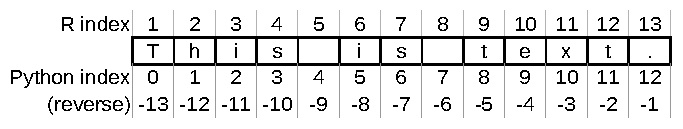
\includegraphics[width=.6\textwidth]{chapter10/text.pdf}\end{center}
  
\doublecodex{chapter10/string}
\doubleoutput{chapter10/string}
\doublecodex{chapter10/manystrings}
\doubleoutput{chapter10/manystrings}

  \caption{Internal representation and of single and multiple texts.'}\label{ex:text}
\end{ccsexample}

As a simple example, the figure at the top of \refex{text} shows how the text `This is a text.' is represented.
This text is split info separate characters, with each character representing a letter (or space, interpunction, emoji or Chinese character).
These characters are indexed starting from the first one, with (as always) R counting from one, but Python counting from zero.

In Python, texts are represented as \fn{str} (string) objects, in which we can directly address the individual characters by their position: \ttt{text[0]} is the first character of \ttt{text}, and so on.
In R, howerver, texts (like all objects) represent columns rather than individual values.
Thus, \ttt{text[1]} in R is the first text in a series of text.
To access individual characters in a text, you have to use a function such as \fn{str\_length} and \fn{str\_sub} that will be discussed in more detail below. 
This also means that in Python, if you have a column (or list) of strings that you need to apply an operation to,
you either need to use one of Panda's methods shown below or use a \concept{for loop} to iterate over all the strings.

\subsection{Methods for dealing with text}

\note{\textbf{R: Stringi, stringr, and base string operations}
  As is so often the case, R has multiple packages that partially replicate functionality for basic text handling.
  In this book we will mainly use the \pkg{stringr} package, which is part of \tidyverse.
  This is not because that package is necessarily better or easier than the alternative \pkg{stringi} package
  or the built-in (\pkg{base}) methods.
  However, the methods are well-documented, clearly named, and consistent with other tidyverse functions,
  so for now it is easiest to stick to \pkg{stringr}.
  In particular, \pkg{stringr} is very similar to \pkg{stringi} (and in fact is partially based on it).
  So, to give one example, the function \fn{str\_detect} is more or less the same as \fn{stringi::str\_detect} and \fn{base::grepl}. 
}
    
The first thing to keep in mind is that once you load any text on R or Python you usually store this content as a \emph{character} or \emph{string} object (or you may also think of \emph{lists} or \emph{dictionaries}, but they will have strings inside anyway), which means that basic operations and conditions of this data type apply, such as indexing or slicing to access individual characters or substrings (see \refsec{datatypes}). In fact, base strings operations are very powerful to clean your text and eliminate a big amount of noise.  Table~\ref{tab:stringoperations} summarises some useful operations on strings in R and Python that will help you in this stage.   

\begin{table}
  \caption{\label{tab:stringoperations}Useful strings operations in R and Python to clean noise}{
  \begin{tabularx}{\textwidth}{lllll}
    \toprule
    String operation      & R (\pkg{stringr})  & Python  & Pandas\\
                          & (whole column)  & (single string) & (whole column)\\     
    \midrule
Count characters in s & \ttt{str\_length(s)}          & \ttt{len(s)}        & \ttt{s.str.len()}  \\
Extract a substring   & \ttt{str\_sub(s, n1, n2)}     & \ttt{s[n1:n2]} & \ttt{s.str.slice(n1, n2)} \\
Test if s contains s2 & \ttt{str\_detect(s, s2)}$^*$       & \ttt{s2 in s}       & \ttt{s.str.match(s2)$^*$} \\
Strip spaces          & \ttt{trimws(s)}               & \ttt{s.strip()}     & \ttt{s.str.strip()} \\
Convert to lowercase  & \ttt{tolower(s)}              & \ttt{s.lower()}     & \ttt{s.str.upper()} \\ 
Convert to uppercase  & \ttt{toupper(s)}              & \ttt{s.upper()}     & \ttt{s.str.lower()} \\ 
Find s1 and replace by s2 & \ttt{str\_replace(s, s1, s2)}$^*$ & \ttt{s.replace(s1, s2)} & \ttt{s.str.replace(s1, s2)$^*$}  \\ 
    \bottomrule
  \end{tabularx}}{(*) The R functions \ttt{str\_detect} and \ttt{str\_replace} and the Pandas function \ttt{s.str.match} and \ttt{s.str.replace} use \concept{regular expressions} to define what to find and replace. See \refsec{regular} below for more information.}
\end{table}

%TODO replace 10.2 by an actual clean with base using stupid .replace(<b>, '') etc. and change explanation here
Let us apply some of these functions/methods to a simple Wikipedia text that contains HTML tags or boilerplate, punctuation and natural upper/lower case letters. Using base function \fn{gsub} in R and \fn{replace} in Python we can remove strings containing specific expressions such as \texttt{<p>} or \texttt{</b>} and include an empty space instead. We can use this same method to eliminate punctuation taking as a reference a pre-defined list of signs (\texttt{:punct:} in base R or the object \texttt{punctuation} from the library \pkg{string} in Python). In the case of converting letters from upper to lower case, we use the base R function \fn{tolower} and the string method \fn{lower} in Python. To remove unnecessary double spaces we apply the base R function \fn{trimws} and method \fn{join} in Python. \refex{clean} shows how to conduct this cleaning process.

\pyrex[output=both,caption=Cleaning text with base functions]{chapter10/clean}
